%!TEX root = ../dissertation_vkslm.tex

\chapter{Handwritten Signature Verification} \label{ch:sig}
In this chapter, we give a brief reference to some essential concepts related to Handwritten Signature Verification, including definitions of notation and terminology used in the following chapters. First, we give an introduction and a general overview of the handwritten signature biometry, afterwards we discuss how an Automatic Handwritten Signature Verification system works, and finally, we give a brief overview of the state-of-the-art on offline signature synthesis based on online data.

\section{Handwritten Signature: a behavioral multimodal biometry}

The term ``Biometrics'' is derived from the Greek word ``bio-metriks''. In which ``bio'' means ``life'' and ``metrics'' means ``to measure''. Biometrics refers to the measurements and statistical analysis of unchanging biological characteristics peculiar to an individual. Biometric systems are
a constantly growing technology \cite{jain2004biometrics} and have been introduced as forms of identification and access control. Biometric identifiers are a unique measurable characteristic used to distinguish and describe individuals \cite{jain2000biometric}. 

Biometric systems are often categorized as physiological or behavioral \cite{ross2008introduction}. The physiological category is characterized by measurements of the body. Examples include fingerprint, palm veins, face recognition, DNA, palm print, hand geometry, iris/retina pattern, and body scent. On the other hand, behavioral biometrics are individual acquired traits and are related to the pattern of behavior of a person. They include typing rhythm, gait, temperament, voice, and handwritten signatures \cite{jain2016}.

Most biometric identifiers require a special type of device for security and control of human identity. However, handwritten signature based biometric systems can be realized requiring no sensor except a pen and a piece of paper. According to \cite{pal2014signature} handwritten signatures can be considered the most legally and socially attributes accepted for person identification. Moreover, the challenge that comes with signature-based authentication is the need for high accuracy results to avoid false authorization or rejection.

Handwritten signature authentication is based on systems for signature verification. 
Whether a given signature belongs to a claimed person or not is decided through a signature verification system, which ultimately strives to learn the manner in which
an individual makes use of their muscular memory (hands,
fingers, and wrist) to reproduce a signature \cite{gupta1997review}. 

A generic handwritten signature based biometric system is shown in Figure \ref{fig_ahsv-overview}. Once the user {\boldm $Y$} deposits the signature, a sensor digitalizes the sample. Later, a feature matrix {\boldm $X$} is built with the information extracted from the input sample. Next, the systems typically have two stages: enrollment {\boldm $X_{E}$} and recognition {\boldm $X_{R}$}. The former builds a system database {\boldm $D$} where the users store their reference signatures as a set of templates, whereas the latter is
used to recognize, identify or verify the identity of a user, who typically claim to be one of the registered users. Then, a score {\boldm $S$} is obtained according to the similarity of the
questioned sample to the claimed template. Finally, the system accepts or rejects the questioned sample.

\begin{figure}[!htb]
\centering
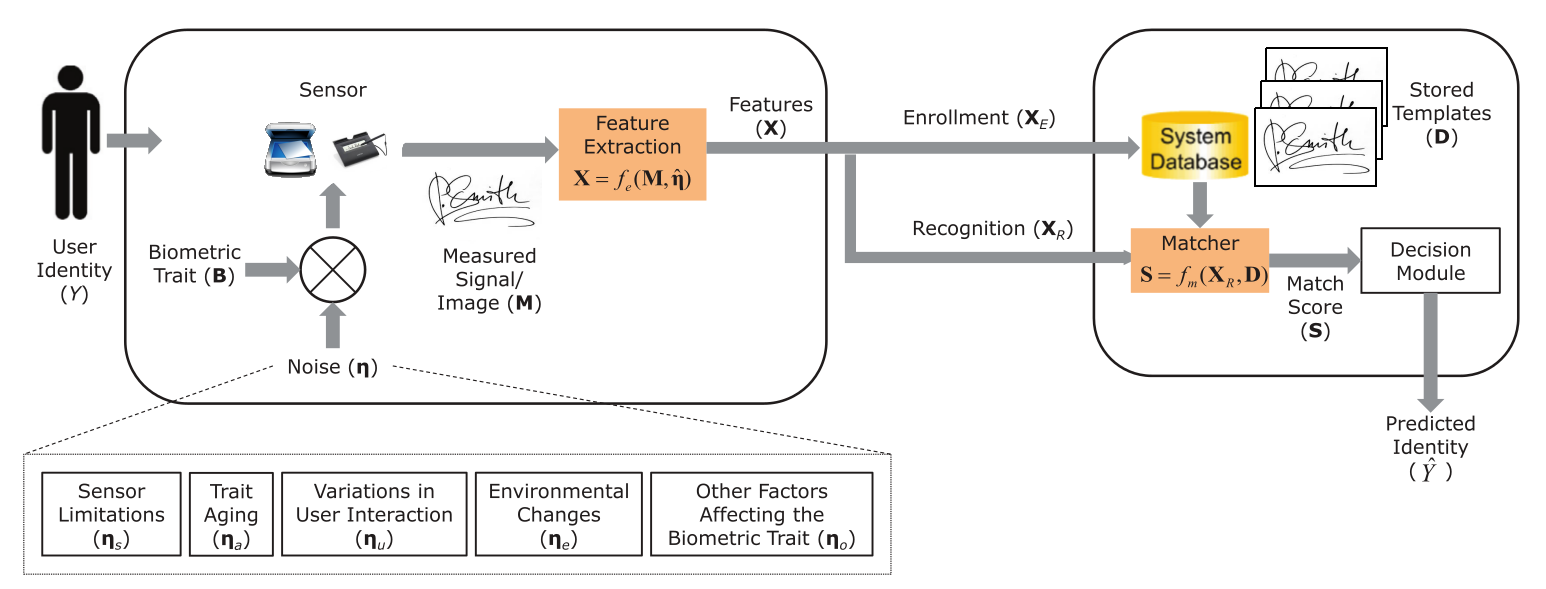
\includegraphics[width=\textwidth]{biometry-overview}
\caption{Overview of a typical handwritten signature based system. Figure adapted from \cite{jain2016}.}
\label{fig_ahsv-overview}
\end{figure}

As Figure \ref{fig_ahsv-overview} shows, the signature acquisition sensor can be either an optical scanner or an acquisition device such as a digitizing tablet. These two different acquisition tools characterize the two classes of signatures, namely: static and dynamic. 

In the static modality, also referred to as offline, an optical scanner is used to obtain the signature directly from the pen on the paper, and only the digital image of the signature is available, see Figure \ref{fig:acquisition} (a). In the dynamic mode, also called online, signatures are acquired through a graphic tablet or a pen-sensitive computer display, see Figure \ref{fig:acquisition} (b). In this mode, data is stored during the writing process and consists of a temporal sequence of the two-dimensional coordinates $(x, y)$ of consecutive points. 

\begin{figure}[!htpb]
\centering
 \subfloat[]{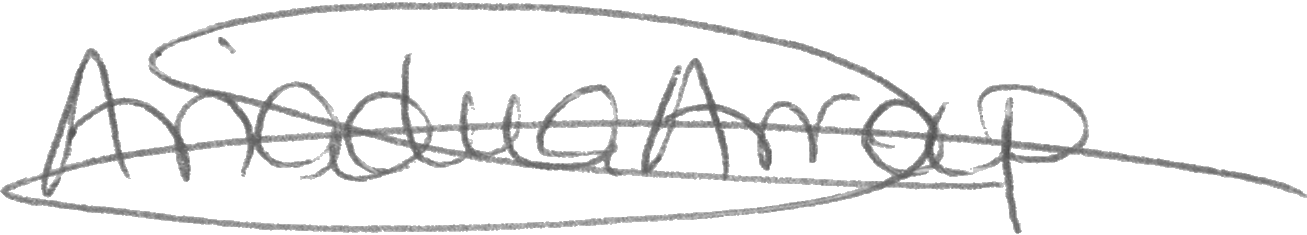
\includegraphics[width=3.2in]{signature.PNG}} 
\hspace*{0.5in} % separation between the subfigures
\subfloat[] {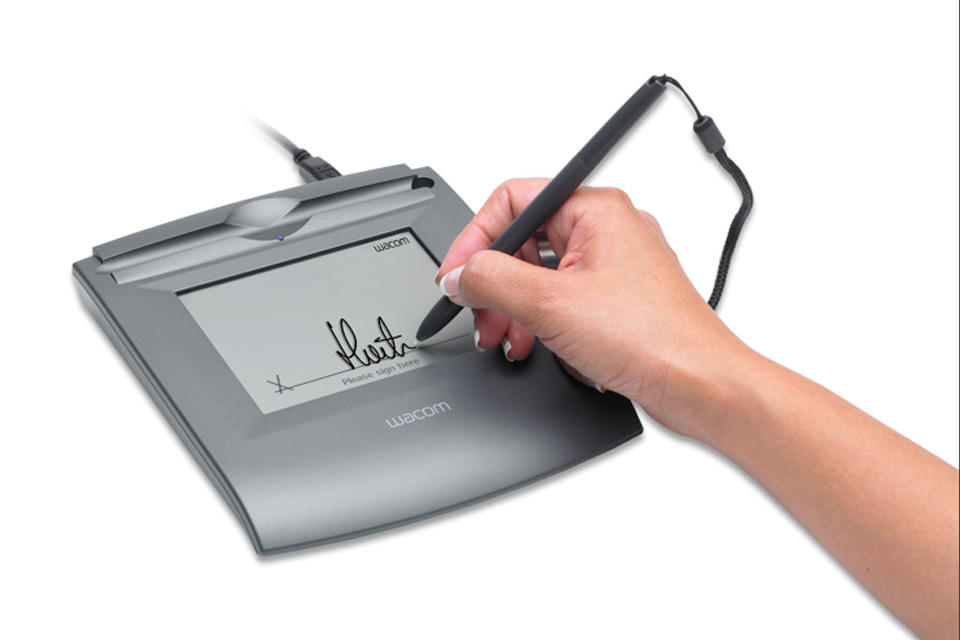
\includegraphics[width=2.7in]{stu500.jpg}}
\caption{Different signature acquisition methods. (a) a signature scanned from paper and (b) digitizing tablet Wacom STU-500 \cite{wacom2016}. } \label{fig:acquisition}
\end{figure}

Specifically, the online modality does not convey information about the overall shape of the signature, the width of the strokes and the texture of the ink on the paper \cite{diaz2014generation}. The offline representation, however, has lost all dynamic information about the manner in which the signature is signed during the acquisition process. As a result, features such as pen trajectory, which can be easily computed in the online domain, can only be inferred from a static image \cite{nel2005estimating}. An example of a colored offline signature and a plotted matching online signature can be found in Figure \ref{fig:offon}. 


\begin{figure}[!htb]
\centering
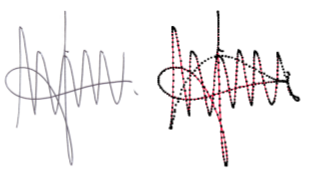
\includegraphics[width=3.8in]{offon}
\caption{An offline and a matching online signature sample. Figure extracted from \cite{sigcomp2009}.}
\label{fig:offon}
\end{figure}

%O pré-processamento tem como objetivos principais a correção de distorções
%geométricas na imagem e a remoção de ruídos, bem como a segmentação que é o
%processo de divisão da assinatura em múltiplas partes. É usualmente utilizada para
%identificar objetos ou outras informações relevantes em representações digitais.
%
%Na fase de classificação, os dados obtidos na extração devem ser utilizados para
%distinguir de forma inteligente entre assinaturas verdadeiras e falsas. Para este fim,
%existem diversas técnicas consagradas, como exemplo podemos citar as Redes Neurais
%Artificiais, HMM, SVM, DTW, entre outros. Além disso, modelos híbridos (junção de
%duas ou mais técnicas) poderão ser investigados para este objetivo.

Once the signature sample is acquired, during the enrollment phase, the system tries to create the subject identity based on behavioral features in the signature. Because of the way we sign, however, it is a subtle task. The rapid movement behind the signature creation is determined by a motor program stored in the brain of each signer applied to tools such as the pen and the paper \cite{pirlo2014advances}. According to \cite{plamondon1989automatic} there is a wide variety of human and social aspects that might affect the way we produce our handwritten signature, it might be influenced by country, age, time, habits, psychological or emotional state. The variability created on the signing process must be taken into account in the signature authentication process.

In fact, the unpredictable intra-personal variability, i.e. the similarity between signatures executed by the same writer, is a crucial challenge of signature-based biometric systems. This variability can be attributed to the several sources of noise ($\eta$) that distort the measured trait. According to Figure \ref{fig_ahsv-overview}, the intra-personal variability affecting the measured sample {\boldm $M$} can be characterized by several variables. These variables include sensor limitations such as resolution or sample rate; biological aging effects or cognitive-motor impairments; user interaction with the sensor; environment changes like background noise and other factors as consequence of the individuals’ mood, hurry or unwillingness to cooperate. The intra-personal variability effect is illustrated in Figure \ref{fig:intraclass}.

\begin{figure}[!h]
\centering
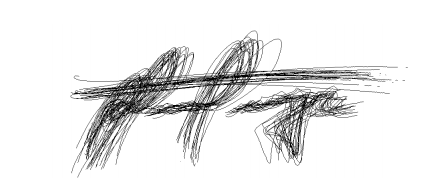
\includegraphics[width=5.2in]{superimposed}
\caption{Superimposed genuine signatures of the same writer. A high intra-personal variability can be noticed. Extracted from \cite{hafemann2015offline}. }
\label{fig:intraclass}
\end{figure}


Another challenge faced by signature-based biometric systems is the unpredictable inter-personal variability, i.e. the similarity between signatures executed by different writers. In a signature-based system, inter-personal variability is mainly attributed to frauds related to malicious people faking the identity of signers. Figure \ref{fig_forgeries} illustrates a visual comparison between genuine signatures and forgeries. 

\begin{figure}[!htb]
\centering
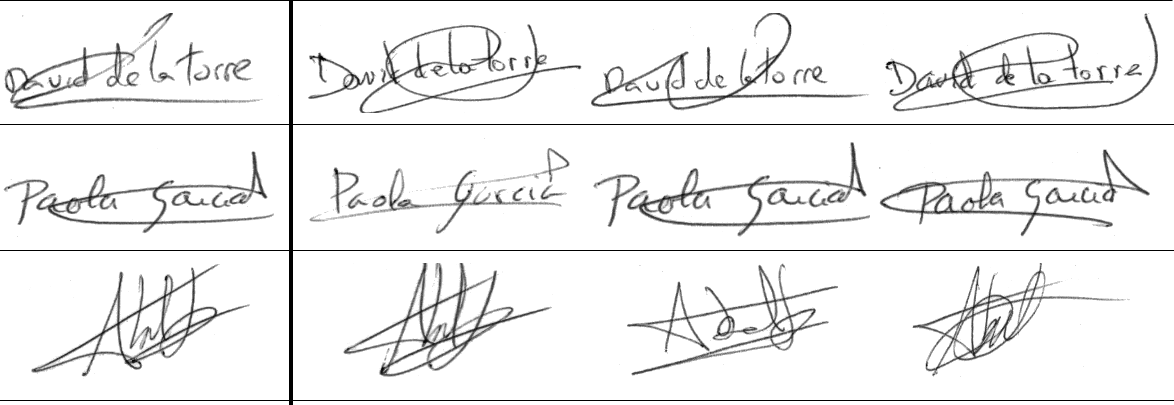
\includegraphics[width=\textwidth]{forgeries}
\caption[The first column of signatures are genuine references, the following three samples are questioned signatures. How many forgeries would you be able to detect? Signature images extracted from \cite{mcyt-100}.]{The first column of signatures are genuine references, the following three samples are questioned signatures. How many forgeries would you be able to detect?\protect\footnotemark Signature images extracted from \cite{mcyt-100}.} 
\label{fig_forgeries}

\end{figure}
\footnotetext{From left to right, top to bottom (F means Forgery and G means Genuine): FGF FFG GFF}

In the field of signature verification, forgeries are generally classified into two types. 
\begin{itemize}
\item The first one is the random forgery which is created in a situation which an impostor who has no information about the person or the shape of the original signature tries to verify the identity of a signer by using his genuine signature. The random forgery test is a typical test used in access control and commercial transactions. 

\item The second type is the skilled forgery, represented by a proper imitation of the genuine signature model. The forger has access for both the user’s name and signature, and learns the signature of a signer and tries to reproduce it with a similar intra-class variability. This test is the most relevant in signature verification for its impact in forensic applications in signature forgery detection. 
 
\end{itemize}




\section{Automatic Handwritten Signature Verification}
An Automatic Handwritten Signature Verification System (AHSVS) is conceptually a pattern recognition application. Pattern recognition is one of the most important and active fields of research. During the past few decades, there has been a considerable growth of interest in problems of pattern recognition, and in the last few years, many methods have been developed in this area, in particular on handwriting recognition and signature verification \cite{book}. 

As any Pattern Recognition system, an AHSVS has three phases: data acquisition and pre-processing, feature extraction and classification \cite{impedovo2008state}.

In the first step, the signatures are acquired and preprocessed, the main goal here is to convert them into a format suitable for the modeling process, correcting geometric distortions and removing noise related to the signature acquisition sensor. Afterwards features are extracted and stored in a knowledge database.  On the classification step, the extracted features are used to distinguish between genuine and forged signatures. Therefore the Signature Verification task is, in essence, a binary classification problem, in which the system's prediction to the input signature sample is either genuine or fraud.

Verification errors occurring in AHSVS are usually categorized as two types \cite{fairhurst1997signature}. On the one hand, a genuine signer may be rejected by the system as a potential impostor (e.g. it could happen when the signer carelessly executes his/her signature), resulting in what is denoted a Type-1 error or False
Rejection. On the other hand, a skilled forger might be able to produce a sample which would be accepted as genuine, resulting in what is called a Type-2 error or False Acceptance. 

In order to improve the performance of signature verification
systems, bigger databases are required. The amount of data available for each user is often
insufficient in real applications. During the enrollment phase,
users are often required to supply only a few samples of their
signatures. In other words, even if there is a significant number
of users enrolled in the system, a classifier needs to perform
well for a new user, for whom only a small set of samples are
available. Since the acquisition
and distribution of real signatures arise legal and privacy
concerns, the use of realistic synthetic signatures could be
regarded as a good alternative. 

\section{Off-line Signature Synthesis Using On-line Samples}

According to \cite{guest2013assessment}, although online samples can be effectively stored as a time-series for use in any form of an automatic system, there are situations where it is needed to output the data into an image reproducing the original static signature. One possible scenario is for human visualization. A legal document (for instance, a driving license or passport) or a bank may require an image-based representation of a signature to
be presented using the data captured as part of a biometric system and stored in a time-series format. There may also be a case where the modality of the signature used for training the user model differs from the signature domain that is being questioned. Although the test sample is of a genuine person, it might not be possible to prove with either an offline or online signature verification system alone. Hence, converting either the training or questioned data into an image reproducing the original static signature would be useful for the development of an integrated version of an offline and online signature verification systems, overcoming the dynamic vs. static dichotomy, unifying the signature biometry \cite{chapter}.

One could synthesize an offline signature 2D image by lineary ``joining the dots''  of
the sample points of the pen trajectory, representing the drawn pen position, in addition to applying some morphological operators to enlarge the tracing to the desired stroke width. However, this may not produce an optimal output in terms of fidelity to the original (i.e. the accuracy of the recreated image when compared against the original signature image). Moreover, the grayscale information would still be missing, which was shown \cite{vargas2010off} to yield better recognition rate results than only the binary offline signature.

The works \cite{ferrer2013realistic, guest2013assessment, rabasse2008new, diaz2014generation} proposed in the literature to generate signature images from online signatures apply different transforms to the dynamic information taking into account the kinematic and the timing order in which the traces were registered, then the samples of the new specimen are interpolated in order to create new images. Thereby, the quality of the synthetic sample is assessed through an offline automatic classifier. Moreover, a method for generating synthetic signatures images has been formulated and experimented to improve the performance of dynamic verifiers \cite{galbally2015line}.


